% This is samplepaper.tex, a sample chapter demonstrating the
% LLNCS macro package for Springer Computer Science proceedings;
% Version 2.20 of 2017/10/04
%
\documentclass[runningheads]{llncs}
\usepackage[english]{babel}

% for in-text and parentheis citations (works with technopress bib style)
\usepackage[round, authoryear]{natbib}
% for hyperlinking cross-references
\usepackage{hyperref}
% For figures
\usepackage{graphicx}
% For block quotes (see https://tex.stackexchange.com/questions/325695/how-to-style-blockquote)
\usepackage{etoolbox}
\usepackage{setspace} % for \onehalfspacing and \singlespacing macros
\AtBeginEnvironment{quote}{\par\singlespacing\small}

% Used for displaying a sample figure. If possible, figure files should
% be included in EPS format.
%
% If you use the hyperref package, please uncomment the following line
% to display URLs in blue roman font according to Springer's eBook style:
% \renewcommand\UrlFont{\color{blue}\rmfamily}

\begin{document}
%
    \title{CS 715 Seminar Thesis}
    \subtitle{Linked Data on the Web}
%
%\titlerunning{Abbreviated paper title}
% If the paper title is too long for the running head, you can set
% an abbreviated paper title here
%
    \author{Lukas M. Loos}
%
%\authorrunning{F. Author et al.}
% First names are abbreviated in the running head.
% If there are more than two authors, 'et al.' is used.
%
    \institute{University of Mannheim}
%
    \maketitle              % typeset the header of the contribution
%
    \begin{abstract}
        The abstract should briefly summarize the contents of the paper in
        150--250 words.

    \end{abstract}
%
%
%


    \section{Available Data}

    \subsection{Linked Open Data}
    When \citet{berners2001semantic} introduced the idea of the semantic web as an evolution of the original document web, their vision was to allow agents to infer the meaning of instances and their relationships published in datasets on the web.
    This is enabled by assigning instances and relations to URIs from standardized vocabularies, making their meaning no more limited to the dataset's scope but globally valid.
    The semantic web relies on various technological standards of which some were specifically developed for it and others already existed.
    Firstly, just like the document web, it relies on HTTP for data transmission.
    RDF~\citep{RDF}, a standard published by the World Wide Web Consortium (W3C) is the recommended language for transferring linked data and describes datasets as collections of triples consisting of subjects, predicates, and objects.
    Vocabularies for linked data are organized in ontologies, defined in the standards RDFS~\citep{RDFS} and OWL~\citep{OWL}.
    Finally, SPARQL~\citep{SPARQL}, another standard by the W3C is a query language that can be used to query linked datasets.

    \subsection{Linked Open Data Cloud}
    Probably the most prominent service around linked open data is the Linked Open Data Cloud (LOD cloud)\footnotemark{}.
    \begin{figure}[ht]
        \centering
        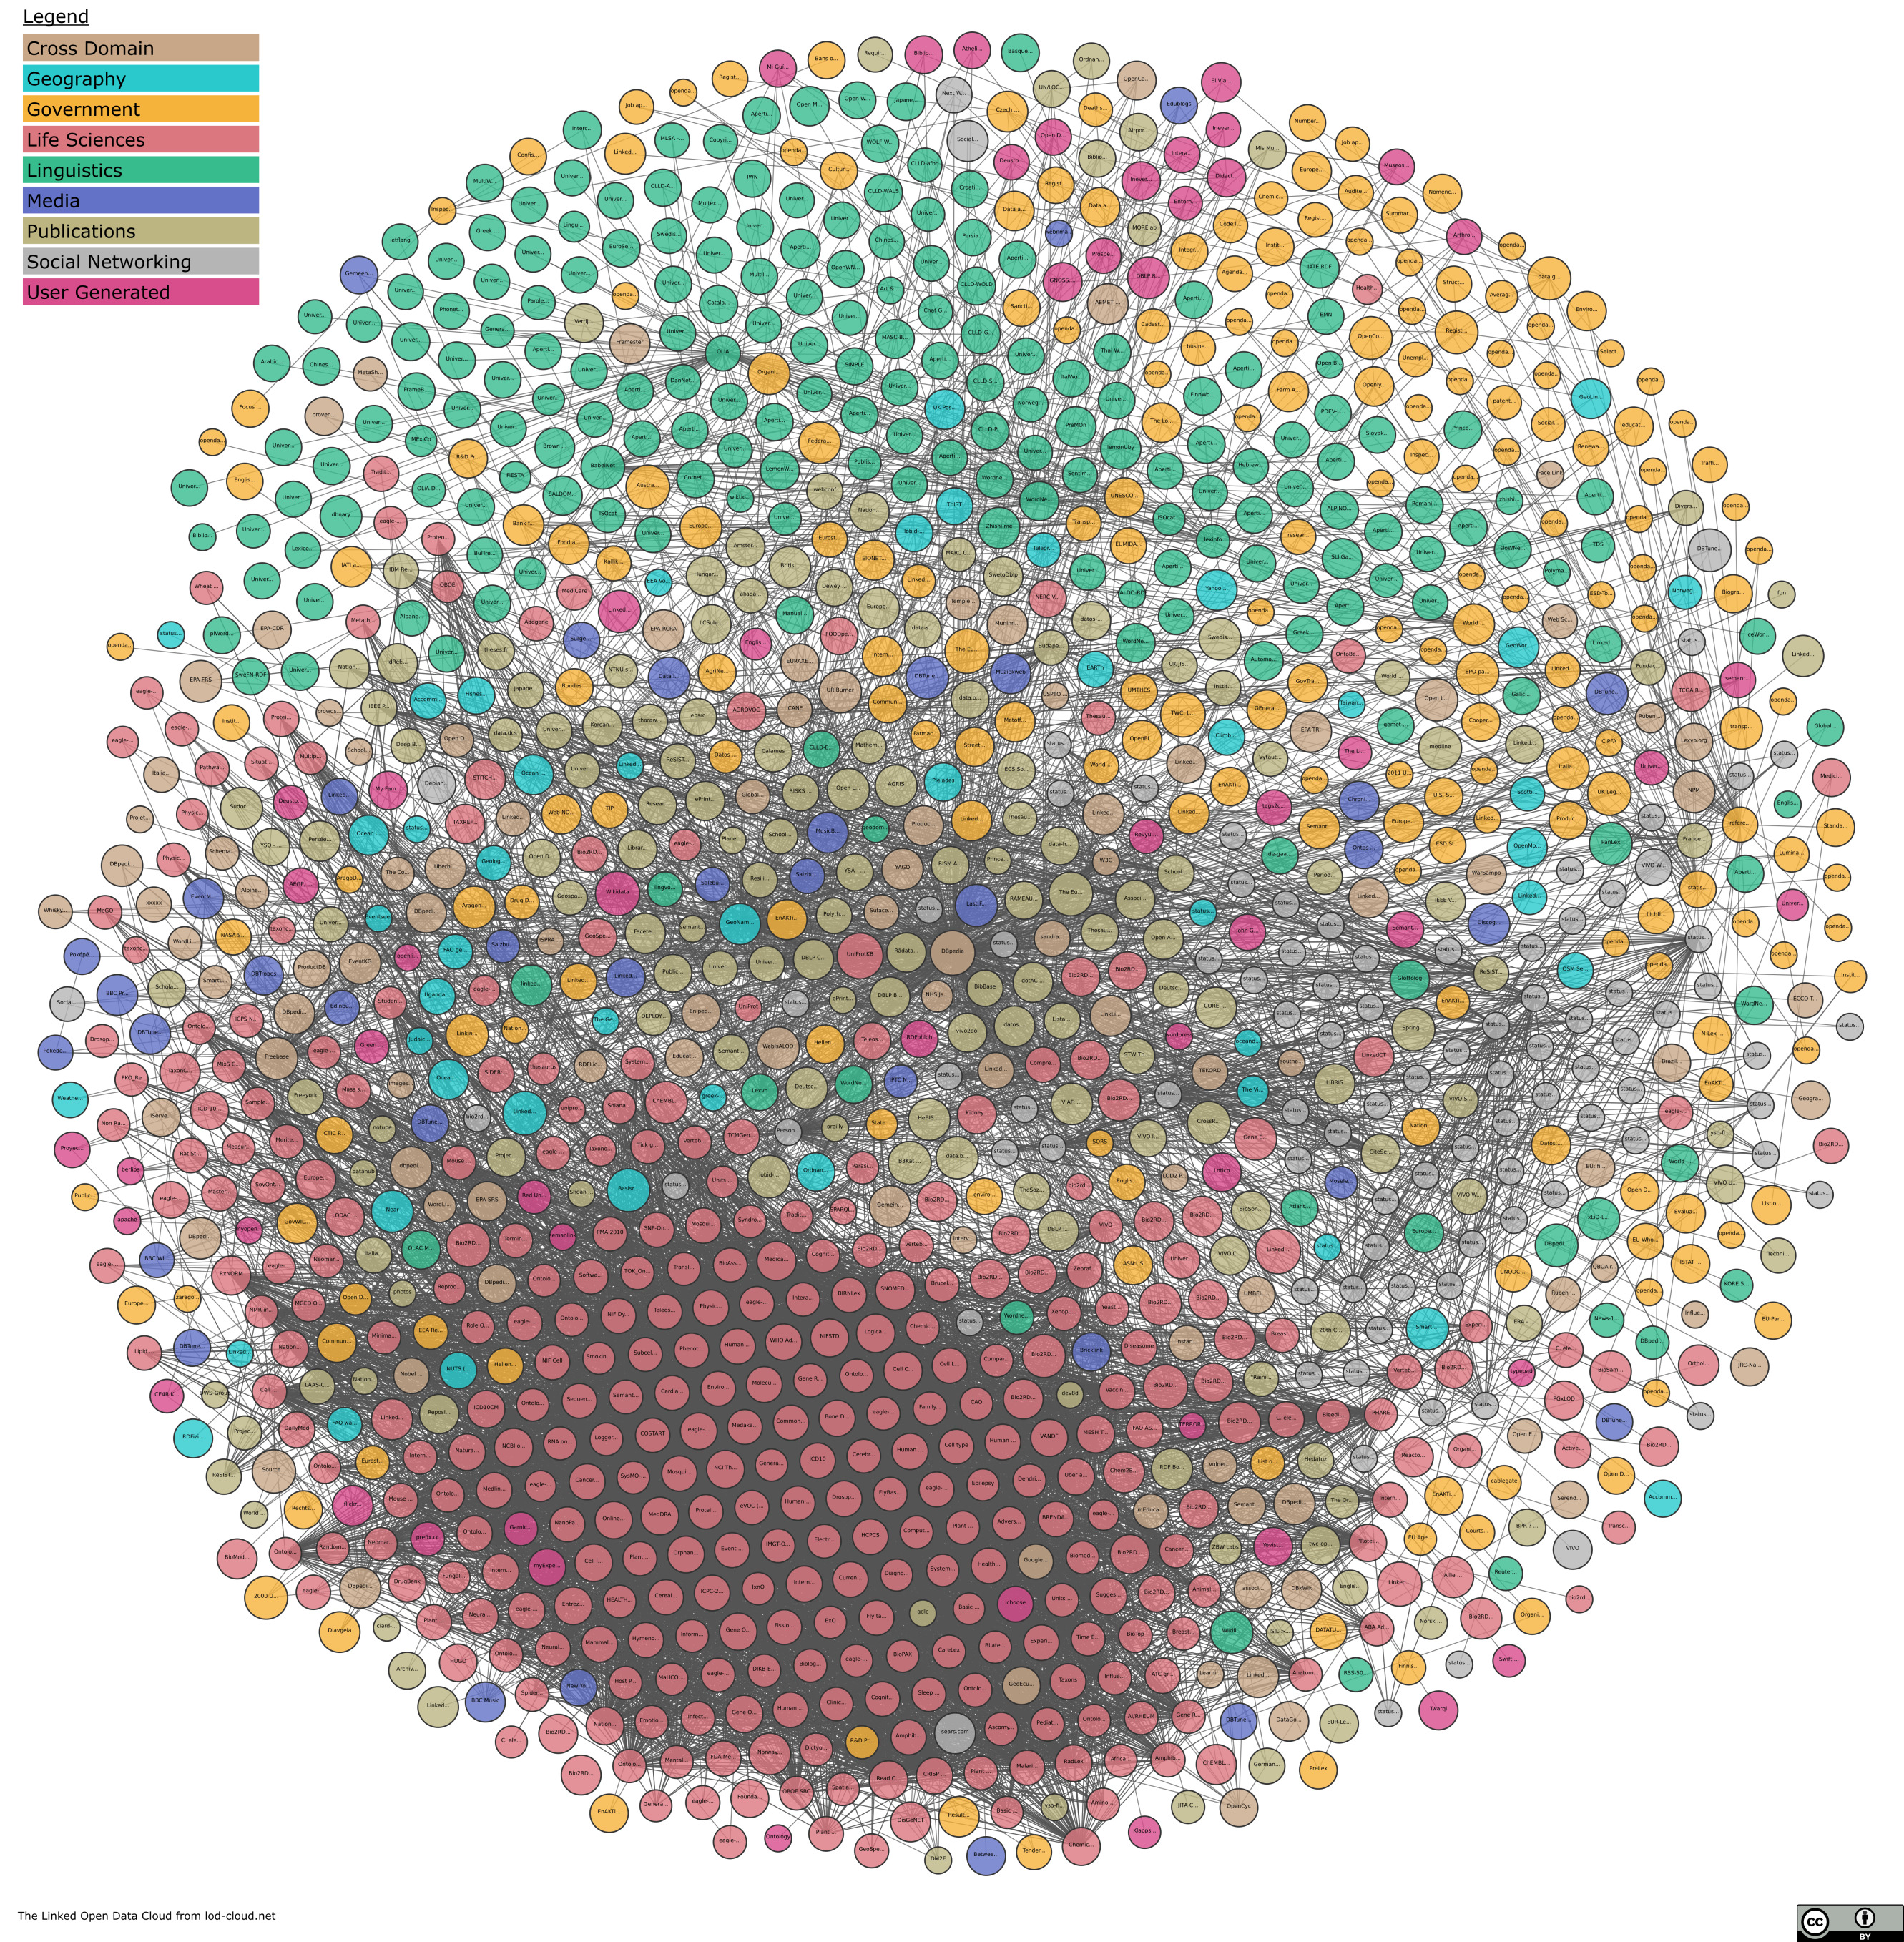
\includegraphics[width=\textwidth]{figures/lod-cloud-sm}
        \caption{The LOD Cloud\protect\footnotemark[\value{footnote}]}
        \label{fig:lod_cloud}
    \end{figure}
    \footnotetext{The Linked Open Data Cloud, https://lod-cloud.net/, (Accessed on 01/06/2022)}
    The LOD cloud is a diagram visualizing linked open datasets and their interconnections.

    For a dataset to be included, it has to meet certain requirements.
    For example, instances have to be annotated with URIs that resolve to RDF data, the dataset must contain at least 1000 triples, and it has to be connected via RDF links to datasets in the diagram with at least 50 links.
    The LOD cloud also provides metadata about the datasets.
    For example, it divides the datasets into different domains, like Media, Government, Publications, Social Networking, or Life Sciences.
    As of May 2021 this catalogue contained 1301 datasets and has become the subject of multiple investigations~\citep{debattista2019lod, kamdar2019enabling, schmachtenberg2014adoption}.

    \subsection{Life Sciences Linked Open Data Cloud}
    In this thesis, I will only take into account datasets from the life sciences domain.
    Biomedical researchers have already been adopting semantic web technologies in their early stages~\citep{ashburner2000gene, bodenreider2004unified, wang2005xml}, motivated by a problem that still exists in the domain and was addressed by Vijay Bulusu, head of data and digital innovation at company Pfizer:
    \begin{quote}
        Vijay Bulusu opened his plenary session at the Bio-IT World Conference \& Expo last week by asking the audience whether - if given \$1 million to spend - they'd buy a machine learning platform or improve the quality of their data.
        Nearly everyone voted for improving data quality.
        Bulusu was pleased.
        Life sciences doesn't really have a big data problem, he explained.
        It has a "lots-of-small-data problem," and data should be our focus~\citep{Pfizer}.
    \end{quote}


    Please note that the first paragraph of a section or subsection is
    not indented.
    The first paragraph that follows a table, figure,
    equation etc. does not need an indent, either.

    Subsequent paragraphs, however, are indented.

    \subsubsection{Sample Heading (Third Level)} Only two levels of
    headings should be numbered. Lower level headings remain unnumbered;
    they are formatted as run-in headings.

    \paragraph{Sample Heading (Fourth Level)}
    The contribution should contain no more than four levels of
    headings. Table~\ref{tab1} gives a summary of all heading levels.

    \begin{table}
        \caption{Table captions should be placed above the
        tables.}\label{tab1}
        \begin{tabular}{|l|l|l|}
            \hline
            Heading level     & Example                                          & Font size and style \\
            \hline
            Title (centered)  & {\Large\bfseries Lecture Notes}                  & 14 point, bold      \\
            1st-level heading & {\large\bfseries 1 Introduction}                 & 12 point, bold      \\
            2nd-level heading & {\bfseries 2.1 Printing Area}                    & 10 point, bold      \\
            3rd-level heading & {\bfseries Run-in Heading in Bold.} Text follows & 10 point, bold      \\
            4th-level heading & {\itshape Lowest Level Heading.} Text follows    & 10 point, italic    \\
            \hline
        \end{tabular}
    \end{table}


    \noindent Displayed equations are centered and set on a separate
    line.
    \begin{equation}
        x + y = z
    \end{equation}
    Please try to avoid rasterized images for line-art diagrams and
    schemas. Whenever possible, use vector graphics instead (see
    Fig.~\ref{fig1}).

    \begin{figure}
        \caption{A figure caption is always placed below the illustration.
        Please note that short captions are centered, while long ones are
        justified by the macro package automatically.} \label{fig1}
    \end{figure}

    \begin{theorem}
        This is a sample theorem. The run-in heading is set in bold, while
        the following text appears in italics. Definitions, lemmas,
        propositions, and corollaries are styled the same way.
    \end{theorem}
%
% the environments 'definition', 'lemma', 'proposition', 'corollary',
% 'remark', and 'example' are defined in the LLNCS documentclass as well.
%
    \begin{proof}
        Proofs, examples, and remarks have the initial word in italics,
        while the following text appears in normal font.
    \end{proof}
    For citations of references, we prefer the use of square brackets
    and consecutive numbers. Citations using labels or the author/year
    convention are also acceptable. The following bibliography provides
    a sample reference list with entries for journal
%
% ---- Bibliography ----
%
% BibTeX users should specify bibliography style 'splncs04'.
% References will then be sorted and formatted in the correct style.
%
    \bibliographystyle{technopress}
    \bibliography{references}
%
\end{document}
